\documentclass[aspectratio=169,xcolor=dvipsnames]{beamer}
% https://github.com/PM25/SimplePlus-BeamerTheme
\usetheme{SimplePlus}

\usepackage{hyperref}
\usepackage{graphicx} 
\usepackage{booktabs}
\usepackage{courier}

\usepackage[spanish]{babel}

% Portada

\title{\large Diseño y desarrollo de un microservicio para la gestión de información de monitorización y predicciones de tráfico en red}

\author{\small \textit{Autor}: Enrique Fernández Sánchez \\
\textit{Tutor}: Pablo Pavón Mariño}

\institute[UPCT]{\\ Universidad Politécnica de Cartagena (UPCT) \\ \vspace{5px}
	
\includegraphics[scale=0.2]{img/escudo_upct.png}
}

\date{\today}

\usepackage{tikz}
\logo{ 
	\begin{tikzpicture}[overlay,remember picture, inner sep=0pt,outer sep=0pt]
		\node[yshift=-20px,left=0.2cm] at (current page.31){
			
\includegraphics[width=3cm]{img/etsit.png}
		};
	\end{tikzpicture}
}

\begin{document}
	% 1
	\begin{frame}
		\titlepage
	\end{frame}

	% 2
	\begin{frame}{Índice}
		\tableofcontents
	\end{frame}

    % --------------------
    \section{Introducción}
    
    \begin{frame}{Introducción}
    
        \begin{itemize}
            \item \textit{Abstract}: Aplicación que permite almacenar muestras de monitorización de tráfico en red, y a su vez, generar predicciones futuras del tráfico de red, en función de la información almacenada.
        \end{itemize}
    
        \begin{block}{Objetivos del proyecto}
            \begin{itemize}
                \item Diseñar una \textbf{aplicación} siguiendo la metodología de \textbf{microservicios}.
                
                \item Investigar herramientas de \textbf{predicción de series temporales}.
                
                \item Investigar \textbf{opciones de almacenamiento} para \textbf{muestras temporales}.
                
                \item Utilizar \textbf{herramientas de documentación} que permitan conocer la estructura de la aplicación.\\
                
            \end{itemize}
        \end{block}
    \end{frame}

	% ---------------------
	
	\section{Tecnologías empleadas}

	\begin{frame}{Microservicios}
		\begin{exampleblock}{Definición de microservicio}
			Sistemas que cumplen las siguientes premisas: 
			
			\begin{itemize}
				\item Sistemas \textbf{pequeños}, \textbf{independientes} y poco ``\textit{acoplados}''. 
				\item \textbf{Código fuente separado} entre los diferentes servicios, no necesariamente mismo lenguaje.
				\item Los servicios \textbf{se comunican} entre sí utilizando \textbf{APIs}.
				\item Cada \textbf{sistema} es \textbf{independiente}, y responsable de su persistencia de datos.
			\end{itemize}
		\end{exampleblock}
		
		\begin{alertblock}{Importancia de utilizar microservicios}
			\begin{itemize}
				\item Permite que otras \textbf{aplicaciones más complejas} puedan \textbf{implementar el servicio} propuesto.
			\end{itemize}
		\end{alertblock}
	\end{frame}

	% ---------------------
	
	\begin{frame}{\texttt{API} \small (\textit{Application Programing Interface})}
		\begin{itemize}
			\item Una API permite a dos \textbf{componentes comunicarse} entre sí \textbf{mediante} una serie de \textbf{reglas}.
			
			\item Supone un ``\textbf{contrato}'' en el que \textbf{se establecen las solicitudes} y respuestas \textbf{esperadas en la comunicación}.
		\end{itemize}
	
		\begin{exampleblock}{Tipos de API}
			Dependiendo de la implementación, distinguimos entre cuatro tipos:
			
			\begin{itemize}
				\item \textbf{SOAP}. Protocolo tradicional, usa mensajes XML (HTTP solo transporte). Ambos interlocutores deben conocer la estructura de los objetos. Poco flexible.
				\item \textbf{RPC}. Basado en llamadas a procedimientos remotos. 
				\item \textbf{WebSocket}. Solución moderna, usa objetos JSON y un canal bidireccional de comunicación.
				\item \textbf{REST}. Solución más popular y flexible. Usa los métodos HTTP. \textbf{Elegimos este tipo}.
			\end{itemize}
		\end{exampleblock}
	\end{frame}
	
	% ---------------------
	
	\begin{frame}{Bases de datos}
		
		\begin{itemize}
			\item En \textbf{función} del \textbf{tipo de dato} a almacenar, se distinguen dos bases de datos dentro de la aplicación:
		\end{itemize}
		
		\begin{columns}
			\begin{column}{0.5\textwidth}
				\begin{block}{Tipo relacional (\texttt{PostgreSQL})}
					\begin{itemize}
						\item Se almacenan \textbf{datos} que puedan tener una \textbf{relación} entre ellos. Por ejemplo: información de una red a monitorizar.
						
						\item Se organizan los datos en una serie de ``\textit{relaciones}'', y estas se almacenan en una o más ``\textit{tablas}''.
						
						\item Cada tabla dispone de una serie de columnas. La información se agrega en forma de filas a la tabla.
					\end{itemize}
				\end{block}
			\end{column}
			
			
			\begin{column}{0.5\textwidth}
				\begin{block}{Tipo serie temporal (\texttt{InfluxDB})}
					\begin{itemize}
						\item Necesario para almacenar \textbf{datos} en forma de \textbf{serie temporal} de manera eficiente.
						
						\item En comparación con el tipo relacional, la fila de datos está identificada por un valor temporal.
						
						\item Algunas ventajas:
						\begin{itemize}
							\item Útil para almacenar datos de telemetría.
							\item Datos comprimidos automáticamente.
							%\item Permite realizar consultas de manera sencilla.							
						\end{itemize}
					\end{itemize}
				\end{block}
			\end{column}
		\end{columns}
	\end{frame}
	
	% ---------------------
	
	\begin{frame}{Lenguaje \& frameworks}
		\begin{columns}
			\begin{column}{0.5\textwidth}
				\begin{exampleblock}{\texttt{Python}}
					Lenguaje de programación orientado a objetos, interpretado y de alto nivel. Muy popular en los siguientes ámbitos:
					
					\begin{itemize}
						\item Aplicaciones web.
						
						\item \textit{Data Science}.
						
						\item Inteligencia Artificial.
					\end{itemize}
					
					\begin{figure}[h!]
						\begin{center}
							
\includegraphics[width=0.7\textwidth]{img/python_logo.png}
							%\caption{asd}
							%\label{img: microservice architecture}
						\end{center}
					\end{figure}
				\end{exampleblock}
			\end{column}
		
			\begin{column}{0.5\textwidth}
				\begin{exampleblock}{\texttt{FastAPI}}
					\textbf{Framework moderno} y rápido para construir \textbf{APIs}. Características:
					
					\begin{itemize}
						\item \textbf{Rápido}: rendimiento equivalente a otros lenguajes (NodeJS o Go).
						\item \textbf{Intuitivo}: soporta autocompletado. 
						\item \textbf{Robusto}: herramienta \texttt{Swagger}/\texttt{ReDoc} automática.
					\end{itemize}
					
					\begin{figure}[h!]
						\begin{center}
							
\includegraphics[width=0.8\textwidth]{img/fastapi_logo.png}
							%\caption{asd}
							%\label{img: microservice architecture}
						\end{center}
					\end{figure}
				\end{exampleblock}
				
				
			\end{column}
		\end{columns}
	\end{frame}

	\begin{frame}{Lenguaje \& frameworks}
		\begin{exampleblock}{\texttt{Prophet}}
			Librería del lenguaje de programación Python, desarrollado por Meta (Facebook). Agrupa una serie de \textbf{procedimientos} que permiten \textbf{realizar predicciones} en un \textbf{dataset temporal}. Características:
			
			\begin{itemize}
				\item Permite encontrar y tener en cuenta \textbf{efectos no lineales} (tendencias diarias, semanales, mensuales...).
				\item Permite predecir datos en \textbf{días vacacionales}.
				\item Basado en inferencia estadística, \textbf{más eficiente} que si utilizáramos técnicas de \textit{Machine Learning}.
			\end{itemize}
			
			\begin{figure}[h!]
				\begin{center}
					
\includegraphics[width=0.4\textwidth]{img/prophet_logo.png}
					%\caption{asd}
					%\label{img: microservice architecture}
				\end{center}
			\end{figure}
		\end{exampleblock}
	\end{frame}
	
	% ---------------------
	
	\begin{frame}{Despliegue en producción}
		Herramientas utilizadas para el despliegue del sistema en un entorno de producción:
		
		\begin{itemize}
			\item \texttt{Docker}. Contenedores.
			\item \texttt{docker-compose}. Despliegue automatizado de contenedores \texttt{Docker}.
			\item \texttt{Traefik}. Enrutador que permite conectar dominios con servicios \texttt{Docker}.
		\end{itemize}
	
		\begin{figure}[h!]
			\begin{center}
				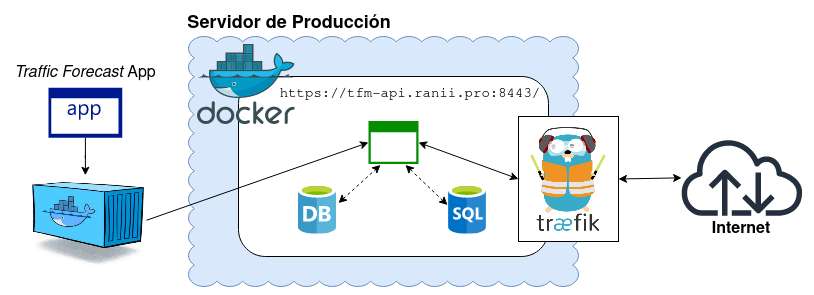
\includegraphics[width=0.95\textwidth]{diag/produccion_tfm.png}
			\end{center}
		\end{figure}
	\end{frame}
	
	% ---------------------
	
	\section{Implementación del sistema}
	
	\begin{frame}{Descripción API REST (I)}
		\begin{columns}
			\begin{column}{0.5\textwidth}
				Para la aplicación se implementan los diferentes agentes utilizando \textbf{dos metodologías}: \\
				
				\vspace{12px}
				
				\begin{enumerate}
					\item \textbf{CRUD} 
					\begin{itemize}
						\item Aquellas que siguen la definición \texttt{Create}, \texttt{Read}, \texttt{Update} \& \texttt{Delete}.
						
						\item \textit{Ejemplo}: redes o interfaces.
					\end{itemize}
				
					\item \textbf{No CRUD}
					\begin{itemize}
						\item Aquellas que no tienen por qué seguir las reglas CRUD.
						
						\item \textit{Ejemplo}: ejecutar predicción de red.
					\end{itemize}
				\end{enumerate}
			\end{column}
		
			\begin{column}{0.5\textwidth}
				\begin{alertblock}{Agentes}
					Se identifican los diferentes ``\textit{agentes}'' presentes en el sistema:
					
					\begin{itemize}
						\item \textbf{Redes} (\texttt{networks}), corresponde con una red que contiene interfaces a monitorizar.
						
						\item \textbf{Interfaces} (\texttt{interfaces}), corresponde con las interfaces de red que queremos monitorizar.
						
						\item \textbf{Muestras de monitorización} (\texttt{samples}). Valor de tráfico asociado a una interfaz en un intervalo determinado.
					\end{itemize}
				\end{alertblock}
			\end{column}
		\end{columns}
	\end{frame}
	
	% ---------------------
	
	\begin{frame}{Descripción API REST (II)}
		
		\textbf{Esquema de la aplicación implementada}
		
		\begin{figure}[h!]
			\begin{center}
				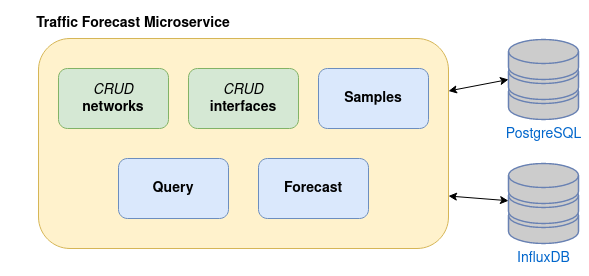
\includegraphics[width=0.75\textwidth]{diag/traffic_forecast_schema.png}
			\end{center}
		\end{figure}
	\end{frame}
	
	% ---------------------
	
	\begin{frame}{Implementación (I)}
		\begin{exampleblock}{\texttt{Factory Pattern}}
			Metodología que \textbf{permite} \textbf{estructurar} un \textbf{proyecto} software de modo que permita:
			\begin{itemize}
				\item \textbf{Añadir} \textbf{funcionalidades} de manera sencilla.
				\item \textbf{Permitir} el \textbf{crecimiento} ordenado de la aplicación.
				\item Ordenar los archivos del proyecto dependiendo de la funcionalidad.
			\end{itemize}
		\end{exampleblock}
	
		\begin{alertblock}{\texttt{ORM} \& \texttt{migrations}}
			\begin{itemize}
				\item \texttt{ORM} (\textit{Object-relational Mappers}). Abstracción de alto nivel que permite \textbf{definir} \textbf{modelos} de datos SQL con el lenguaje \textbf{Python}.
				
				\item \texttt{migrations}. Permite tener un \textbf{control} de \textbf{versiones} dentro de los \textbf{modelos} de datos de la aplicación. Facilita el despliegue de la base de datos, en lo que a estructura de tablas se refiere.	
		\end{itemize}
		\end{alertblock}
		
	\end{frame}

	\begin{frame}{Implementación (II)}
		\begin{columns}
			\begin{column}{0.6\textwidth}
				\textbf{Estructura de ficheros del proyecto}
				
				\begin{itemize}
					\item \texttt{migrations}. Contiene las versiones de la DB.
					
					\item \texttt{src}
					
					\begin{itemize}
						\item \texttt{crud}. Funcionalidad de agentes CRUD.
						
						\item \texttt{database}. Contiene modelos de datos SQL.
						
						\item \texttt{noncrud} Funcionalidad agentes no CRUD.
						
						\item \texttt{routes}. Rutas de la aplicación.
						
						\item \texttt{schemas}. Esquema de datos.
						
						\item \texttt{utils}. Utilidades, \texttt{wrapper InfluxDB}.
						
						\item \texttt{config.py}. Configuración app.
						
						\item \texttt{main.py}. Archivo principal.
					\end{itemize}
				
					\item \texttt{Dockerfile}. Instrucciones para contenedor Docker.
					
					\item \texttt{requirements.txt}. Módulos Python utilizados.
				\end{itemize}
			\end{column}
		
			\begin{column}{0.4\textwidth}
				\begin{figure}[h!]
					\begin{center}
						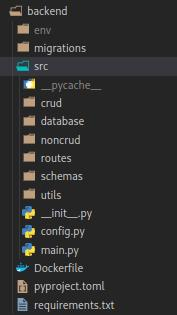
\includegraphics[width=0.65\textwidth]{img/folder_structure.jpg}
					\end{center}
				\end{figure}
			\end{column}
		\end{columns}
	\end{frame}
	
	% ---------------------
	
	\begin{frame}{OpenAPI. \texttt{Swagger} \& \texttt{ReDoc}}
		\begin{itemize}
			\item FastAPI permite \textbf{generar de manera automática} una serie de rutas que sirven como \textbf{documentación del proyecto}.
			
			\item En estas herramientas se muestran al usuario la información de: 
			
			\begin{itemize}
				\item Rutas de la aplicación.
				
				\item Parámetros de entrada y de salida para una petición.
				
				\item Modelos de datos para cada una de las rutas.
				
				\item Posibles códigos HTTP de respuesta para las peticiones.
			\end{itemize}
		
			\item \textbf{Permite} al usuario \textbf{realizar peticiones al servidor} y ver su resultado, desde la misma herramienta.
		\end{itemize}
		
		\begin{block}{Acceso a las herramientas de documentación}
			\begin{itemize}
				\item \textbf{Swagger}: \href{https://tfm-api.ranii.pro:8443/docs}{\texttt{https://tfm-api.ranii.pro:8443/docs}}
				
				\item \textbf{ReDoc}: \href{https://tfm-api.ranii.pro:8443/redoc}{\texttt{https://tfm-api.ranii.pro:8443/redoc}}
			\end{itemize}
		\end{block}
	\end{frame}
	
	% ---------------------
	
	\begin{frame}{Modelos de datos. \texttt{SQL}}
		
		\begin{itemize}
			\item Definimos los datos y su \textbf{representación dentro} de nuestra \textbf{aplicación}.
			
			\item \textbf{En función} del \textbf{tipo de dato}, almacenaremos en \textbf{base de datos tipo relacional} (\texttt{SQL}) o \textbf{base de datos tipo serie temporal} (\texttt{InfluxDB}).
		\end{itemize}

		\vspace{11px}

		\textbf{Tablas utilizadas en la base de datos SQL}

		\begin{columns}
			\begin{column}{0.5\textwidth}
				\begin{table}[h!]
					\centering
					\begin{tabular}{|l|}
						\hline
						\multicolumn{1}{|c|}{\textit{\textbf{Networks}}} \\ \hline
						\texttt{id\_network}: Int, Public Key, Unique                 \\ \hline
						\texttt{name}: String                                     \\ \hline
						\texttt{description}: String                              \\ \hline
						\texttt{ip\_red}: String                                  \\ \hline
						\texttt{influx\_net}: String                              \\ \hline
					\end{tabular}
					%\caption{Modelo de datos para las redes a monitorizar. Equivale con la tabla \textit{networks}.}
					%\label{tab: modelo sql networks}
				\end{table}
			\end{column}
		
			\begin{column}{0.5\textwidth}
				\begin{table}[h!]
					\centering
					\begin{tabular}{|l|}
						\hline
						\multicolumn{1}{|c|}{\textit{\textbf{Interfaces}}} \\ \hline
						\texttt{id\_interface}: Int, Public Key, Unique             \\ \hline
						\texttt{name}: String                                       \\ \hline
						\texttt{description}: String                                \\ \hline
						\texttt{influx\_if\_rx}: String                             \\ \hline
						\texttt{influx\_if\_tx}: String                             \\ \hline
						\texttt{network}: Int, Foreign Key                          \\ \hline
					\end{tabular}
					%\caption{Modelo de datos para las interfaces a monitorizar. Equivale con la tabla \textit{interfaces}.}
					%\label{tab: modelo sql interfaces}
				\end{table}
			\end{column}
		\end{columns}
	\end{frame}

	\begin{frame}{Modelos de datos. \texttt{InfluxDB}}
		\begin{itemize}
			\item En \texttt{InfluxDB} almacenamos las muestras de tráfico en red.
		\end{itemize}
	
		\vspace{11px}
	
		\textbf{Configuración InfluxDB para el sistema}
	
		\begin{table}[]
			\centering
			\begin{tabular}{|c|c|}
				\hline
				\textbf{InfluxDB}    & \textbf{Descripción}                                                                                                                            \\ \hline
				\texttt{measurement} & \begin{tabular}[c]{@{}c@{}}Red a monitorizar, \\ valor almacenado en \texttt{Networks::influx\_net}\end{tabular}                                         \\ \hline
				\texttt{fields}      & Nombre del valor a monitorizar (\textit{link\_count})                                                                                                    \\ \hline
				\texttt{tags}        & \begin{tabular}[c]{@{}c@{}}Solo disponemos un \texttt{tag}, llamado \texttt{interface}, \\ contiene la información del identificador de una interfaz\end{tabular} \\ \hline
				\texttt{points}      & Corresponde con el valor numérico del campo \texttt{field}.                                                                                              \\ \hline
			\end{tabular}
			%\caption{}
			%\label{tab:my-table}
		\end{table}
	
	\end{frame}
	
	% ---------------------
	
	\begin{frame}{Predicción de tráfico de red (I)}
		\begin{itemize}
			\item El sistema es \textbf{capaz} de \textbf{ejecutar predicciones} de tráfico de red, en función de las \textbf{muestras de monitorización} previamente \textbf{almacenadas en el sistema}.
		\end{itemize}
	
		\begin{exampleblock}{Pasos para realizar una predicción de tráfico}
			\begin{enumerate}
				\item \textbf{Creamos una red} a monitorizar. \texttt{POST} a \texttt{/networks}.
				
				\item \textbf{Creamos una interfaz} a monitorizar. \texttt{POST} a \texttt{/networks/<net>/interfaces}.
				
				\item \textbf{Importamos datos} de monitorización.  Dos maneras: 
				\begin{itemize}
					\item \texttt{POST} a ruta: \texttt{/samples/<net>/import\_topology}.
					
					\item \texttt{POST} a ruta: \texttt{/samples/<net>/import\_interface/<if>}.
				\end{itemize}
			
				\item \textbf{Ejecutamos predicción de tráfico} en red. Configuramos la predicción y lanzamos la petición \texttt{POST} a \texttt{/forecast}.
			\end{enumerate}
		\end{exampleblock}
	\end{frame}
	
	% ---------------------
	
	\begin{frame}{Predicción de tráfico de red (II)}
		\begin{columns}
			\begin{column}{0.4\textwidth}
				\begin{figure}[h!]
					\begin{center}
						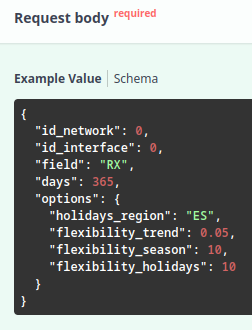
\includegraphics[width=0.9\textwidth]{img/parameters_post_forecast.png}
					\end{center}
				\end{figure}
			\end{column}
		
			\begin{column}{0.6\textwidth}
				\textbf{Parámetros para la ejecución de la predicción de tráfico}
				
				\begin{itemize}
					\item \texttt{field}. Campo para elegir si RX o TX.
					
					\item \texttt{days}. Número de días a predecir.
					
					\item \texttt{options}. Opciones que modifican la flexibilidad de la predicción:
					\begin{itemize}
						\item \texttt{holidays\_region}
						\item \texttt{flexibility\_trend}
						\item \texttt{flexibility\_season}
						\item \texttt{flexibility\_holidays}
					\end{itemize}
				\end{itemize}
			\end{column}
		\end{columns}
	\end{frame}
	
	% ---------------------
	
	\begin{frame}{Resumen rutas HTTP (I)}
		\begin{columns}
			\begin{column}{0.5\textwidth}
				\begin{block}{\textbf{CRUD}: \texttt{networks} (\texttt{/networks})}
					\begin{itemize}
						\item \textbf{Información} de \textbf{todas} las redes: \\ \textit{GET} - \texttt{/networks}
						
						\item \textbf{Crear} una red: \\ \textit{POST} - \texttt{/networks}
						
						\item \textbf{Información} de \textbf{una} red: \\ \textit{GET} - \texttt{/networks/<net\_id>}
						
						\item \textbf{Eliminar} una red: \\ \textit{DELETE} - \texttt{/networks/<net\_id>}
						
						\item \textbf{Actualizar} una red: \\ \textit{PATCH} - \texttt{/networks/<net\_id>}
					\end{itemize}
				\end{block}
			\end{column}
		
			\begin{column}{0.5\textwidth}
				\begin{block}{\textbf{CRUD}: \texttt{interfaces} (\texttt{/networks/<id1>/interfaces})}
					\begin{itemize}
						\item \textbf{Información} de \textbf{todas} las interfaces: \\ \textit{GET} - \texttt{\small /networks/id/interfaces}
						
						\item \textbf{Crear} una interfaz: \\ \textit{POST} - \texttt{\small /networks/id/interfaces}
						
						\item \textbf{Información} de \textbf{una} interfaz: \\ \textit{GET} - \texttt{/../interfaces/<id2>}
						
						\item \textbf{Eliminar} una interfaz: \\ \textit{DELETE} - \texttt{/../interfaces/<id2>}
						
						\item \textbf{Actualizar} una interfaz: \\ \textit{PATCH} - \texttt{/../interfaces/<id2>}
					\end{itemize}
				\end{block}
			\end{column}
		
		\end{columns}
	\end{frame}

	\begin{frame}{Resumen rutas HTTP (II)}
		\begin{columns}
			\begin{column}{0.5\textwidth}
				\begin{exampleblock}{\texttt{Samples}}
					\begin{itemize}
						\item \textbf{Importar} datos de topología con \textbf{más de una interfaz}: \\ \textit{\small POST} - \texttt{\small /samples/id/import\_topology}
						
						\item \textbf{Importar} datos de \textbf{una interfaz}: \\ \textit{POST} - \texttt{\small /samples/id/import\_interface/id}
					\end{itemize}
				\end{exampleblock}
			\end{column}
		
			\begin{column}{0.5\textwidth}
				\begin{exampleblock}{\texttt{Query Samples}}
					\begin{itemize}
						\item \textbf{Consultar} \textbf{datos} de monitorización \textbf{almacenados}: \\ \textit{GET} - \texttt{\small /query/}
					\end{itemize}
				\end{exampleblock}
			
				\begin{exampleblock}{\texttt{Forecast}}
					\begin{itemize}
						\item \textbf{Ejecutar} \textbf{predicción} de tráfico en red: \\ \textit{POST} - \texttt{\small /forecast/}
					\end{itemize}
				\end{exampleblock}
			\end{column}
		\end{columns}
	\end{frame}
	
	% ---------------------
	
	\section{Validación del sistema}
	
	\begin{frame}{Validación del sistema (I)}
		Para demostrar el funcionamiento del sistema, se realiza una \textbf{batería de pruebas} de las funcionalidades implementadas. Dichas pruebas son:
		
		\begin{enumerate}
			\item \textbf{Crear una red} a monitorizar.
			
			\item \textbf{Crear una interfaz} dentro de una red a monitorizar.
			
			\item \textbf{Cargar muestras} en interfaz de red.
			
			\item Cargar una topología de red sobre una red a monitorizar.
			
			\item \textbf{Consultar datos} de monitorización.
			
			\item \textbf{Ejecutar una predicción} de un año.
		\end{enumerate}
	
	\vspace{12px}
	
	Estas pruebas corresponden con las \textbf{pruebas unitarias} del sistema.
		
	\end{frame}

	\begin{frame}{Validación del sistema (II)}
		\begin{columns}
			\begin{column}{0.52\textwidth}
				\begin{block}{Demo! (\textit{2 minutos})}
					Realizamos una validación del sistema.
					
					\vspace{12px}
					
					\href{https://tfm-api.ranii.pro:8443/docs}{\small \texttt{https://tfm-api.ranii.pro:8443/docs}}
					
					\vspace{12px}
					 
					\begin{itemize}
						\item \textit{Objetivo}: Completar una predicción de un año. 
						\item \textit{Requisito}: Asumir sistema sin datos almacenados.
						\item \textit{Resultado}: Una predicción similar a la de la figura.
					\end{itemize}
				\end{block}
			\end{column}
		
			\begin{column}{0.5\textwidth}
				\begin{figure}[h!]
					\begin{center}
						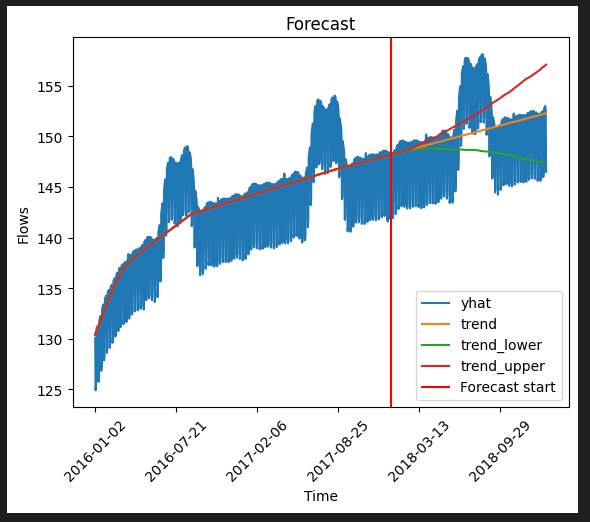
\includegraphics[width=1\textwidth]{img/graph_forecast_2.png}
					\end{center}
				\end{figure}
			\end{column}
		\end{columns}
	\end{frame}
	
	% ---------------------
	
	\section{Conclusiones}
	
	\begin{frame}{Conclusiones}
		\begin{itemize}
			\item Alcanzados todos los objetivos propuestos.
			
			\item Se ha desarrollado una \textbf{microservicio completo}, permitiendo ser implementado por otras aplicaciones.
			
			\item El sistema es \textbf{capaz} de \textbf{almacenar} muestras de monitorización, además de poder \textbf{generar predicciones} de tráfico en red en la escala temporal que el usuario solicite.
		\end{itemize}
	
		\begin{exampleblock}{Propuestas futuras}
			\begin{itemize}
				\item Permitir la \textbf{importación} de \textbf{datos de monitorización} de \textbf{herramientas específicas} de planificación de red.
				
				\item Añadir \textbf{funcionalidad de SSE} (\textit{Server Side Event}) para \textbf{tareas} que requieran un \textbf{largo tiempo de ejecución}.
				
				\item Extender la funcionalidad de las \textbf{predicciones}, permitiendo tener una selección \textbf{más selectiva}, o añadir \textbf{filtrados extra}.
			\end{itemize}
		\end{exampleblock}
	\end{frame}
	
	% ---------------------
	
	\section{Bibliografía}
	
	\begin{frame}{Bibliografía}
		\begin{itemize}
		    \item La contenida en la memoria del proyecto: páginas 53 - 54
		\end{itemize}
	\end{frame}
	
	\begin{frame}
	    \begin{center}
	        \vspace{30px}
	        \Large \textbf{Muchas gracias por su atención} \\
	        \vspace{30px}
	        \large ¿Preguntas? \\
	        \vspace{60px}
	        
	        Enlace a la aplicación: \\
	        \href{https://tfm-api.ranii.pro:8443/docs}{\texttt{https://tfm-api.ranii.pro:8443/}}
	    \end{center}
	\end{frame}
	
\end{document}